% Options for packages loaded elsewhere
\PassOptionsToPackage{unicode}{hyperref}
\PassOptionsToPackage{hyphens}{url}
%
\documentclass[
]{article}
\usepackage{lmodern}
\usepackage{amssymb,amsmath}
\usepackage{ifxetex,ifluatex}
\ifnum 0\ifxetex 1\fi\ifluatex 1\fi=0 % if pdftex
  \usepackage[T1]{fontenc}
  \usepackage[utf8]{inputenc}
  \usepackage{textcomp} % provide euro and other symbols
\else % if luatex or xetex
  \usepackage{unicode-math}
  \defaultfontfeatures{Scale=MatchLowercase}
  \defaultfontfeatures[\rmfamily]{Ligatures=TeX,Scale=1}
\fi
% Use upquote if available, for straight quotes in verbatim environments
\IfFileExists{upquote.sty}{\usepackage{upquote}}{}
\IfFileExists{microtype.sty}{% use microtype if available
  \usepackage[]{microtype}
  \UseMicrotypeSet[protrusion]{basicmath} % disable protrusion for tt fonts
}{}
\makeatletter
\@ifundefined{KOMAClassName}{% if non-KOMA class
  \IfFileExists{parskip.sty}{%
    \usepackage{parskip}
  }{% else
    \setlength{\parindent}{0pt}
    \setlength{\parskip}{6pt plus 2pt minus 1pt}}
}{% if KOMA class
  \KOMAoptions{parskip=half}}
\makeatother
\usepackage{xcolor}
\IfFileExists{xurl.sty}{\usepackage{xurl}}{} % add URL line breaks if available
\IfFileExists{bookmark.sty}{\usepackage{bookmark}}{\usepackage{hyperref}}
\hypersetup{
  hidelinks,
  pdfcreator={LaTeX via pandoc}}
\urlstyle{same} % disable monospaced font for URLs
\usepackage[margin=1in]{geometry}
\usepackage{color}
\usepackage{fancyvrb}
\newcommand{\VerbBar}{|}
\newcommand{\VERB}{\Verb[commandchars=\\\{\}]}
\DefineVerbatimEnvironment{Highlighting}{Verbatim}{commandchars=\\\{\}}
% Add ',fontsize=\small' for more characters per line
\usepackage{framed}
\definecolor{shadecolor}{RGB}{248,248,248}
\newenvironment{Shaded}{\begin{snugshade}}{\end{snugshade}}
\newcommand{\AlertTok}[1]{\textcolor[rgb]{0.94,0.16,0.16}{#1}}
\newcommand{\AnnotationTok}[1]{\textcolor[rgb]{0.56,0.35,0.01}{\textbf{\textit{#1}}}}
\newcommand{\AttributeTok}[1]{\textcolor[rgb]{0.77,0.63,0.00}{#1}}
\newcommand{\BaseNTok}[1]{\textcolor[rgb]{0.00,0.00,0.81}{#1}}
\newcommand{\BuiltInTok}[1]{#1}
\newcommand{\CharTok}[1]{\textcolor[rgb]{0.31,0.60,0.02}{#1}}
\newcommand{\CommentTok}[1]{\textcolor[rgb]{0.56,0.35,0.01}{\textit{#1}}}
\newcommand{\CommentVarTok}[1]{\textcolor[rgb]{0.56,0.35,0.01}{\textbf{\textit{#1}}}}
\newcommand{\ConstantTok}[1]{\textcolor[rgb]{0.00,0.00,0.00}{#1}}
\newcommand{\ControlFlowTok}[1]{\textcolor[rgb]{0.13,0.29,0.53}{\textbf{#1}}}
\newcommand{\DataTypeTok}[1]{\textcolor[rgb]{0.13,0.29,0.53}{#1}}
\newcommand{\DecValTok}[1]{\textcolor[rgb]{0.00,0.00,0.81}{#1}}
\newcommand{\DocumentationTok}[1]{\textcolor[rgb]{0.56,0.35,0.01}{\textbf{\textit{#1}}}}
\newcommand{\ErrorTok}[1]{\textcolor[rgb]{0.64,0.00,0.00}{\textbf{#1}}}
\newcommand{\ExtensionTok}[1]{#1}
\newcommand{\FloatTok}[1]{\textcolor[rgb]{0.00,0.00,0.81}{#1}}
\newcommand{\FunctionTok}[1]{\textcolor[rgb]{0.00,0.00,0.00}{#1}}
\newcommand{\ImportTok}[1]{#1}
\newcommand{\InformationTok}[1]{\textcolor[rgb]{0.56,0.35,0.01}{\textbf{\textit{#1}}}}
\newcommand{\KeywordTok}[1]{\textcolor[rgb]{0.13,0.29,0.53}{\textbf{#1}}}
\newcommand{\NormalTok}[1]{#1}
\newcommand{\OperatorTok}[1]{\textcolor[rgb]{0.81,0.36,0.00}{\textbf{#1}}}
\newcommand{\OtherTok}[1]{\textcolor[rgb]{0.56,0.35,0.01}{#1}}
\newcommand{\PreprocessorTok}[1]{\textcolor[rgb]{0.56,0.35,0.01}{\textit{#1}}}
\newcommand{\RegionMarkerTok}[1]{#1}
\newcommand{\SpecialCharTok}[1]{\textcolor[rgb]{0.00,0.00,0.00}{#1}}
\newcommand{\SpecialStringTok}[1]{\textcolor[rgb]{0.31,0.60,0.02}{#1}}
\newcommand{\StringTok}[1]{\textcolor[rgb]{0.31,0.60,0.02}{#1}}
\newcommand{\VariableTok}[1]{\textcolor[rgb]{0.00,0.00,0.00}{#1}}
\newcommand{\VerbatimStringTok}[1]{\textcolor[rgb]{0.31,0.60,0.02}{#1}}
\newcommand{\WarningTok}[1]{\textcolor[rgb]{0.56,0.35,0.01}{\textbf{\textit{#1}}}}
\usepackage{graphicx,grffile}
\makeatletter
\def\maxwidth{\ifdim\Gin@nat@width>\linewidth\linewidth\else\Gin@nat@width\fi}
\def\maxheight{\ifdim\Gin@nat@height>\textheight\textheight\else\Gin@nat@height\fi}
\makeatother
% Scale images if necessary, so that they will not overflow the page
% margins by default, and it is still possible to overwrite the defaults
% using explicit options in \includegraphics[width, height, ...]{}
\setkeys{Gin}{width=\maxwidth,height=\maxheight,keepaspectratio}
% Set default figure placement to htbp
\makeatletter
\def\fps@figure{htbp}
\makeatother
\setlength{\emergencystretch}{3em} % prevent overfull lines
\providecommand{\tightlist}{%
  \setlength{\itemsep}{0pt}\setlength{\parskip}{0pt}}
\setcounter{secnumdepth}{-\maxdimen} % remove section numbering

\author{}
\date{\vspace{-2.5em}}

\begin{document}

\hypertarget{shellchron}{%
\section{ShellChron}\label{shellchron}}

\href{https://travis-ci.com/nielsjdewinter/ShellChron}{\includegraphics{https://travis-ci.com/nielsjdewinter/ShellChron.svg?branch=master}}

The ShellChron package contains all formulae and documentation required
to run the ShellChron model. The ShellChron model uses stable oxygen
isotope records (d18O) from seasonal paleo-archives to create an age
model for the archive.

In short, ShellChron feeds a temperature sinusoid (Figure 1; see details
in ``temperature\_curve()'' function) and a skewed growth rate sinusoid
(Figure 2; see details in ``growth\_rate\_curve()'' function) to a d18O
model (see details in ``d18O\_model()'' function). The resulting
modelled d18O is then compared with the user-provided d18O data and the
parameters of the temperature and growth rate functions are optimized
using the SCEUA algorithm (see
\href{https://doi.org/10.1029/91WR02985}{Duan et al., 1992}) to match
the d18O data. As a result, the timing of each data point with reference
to the seasonal cycle is exported, from which an age model for the
entire record can be constructed.

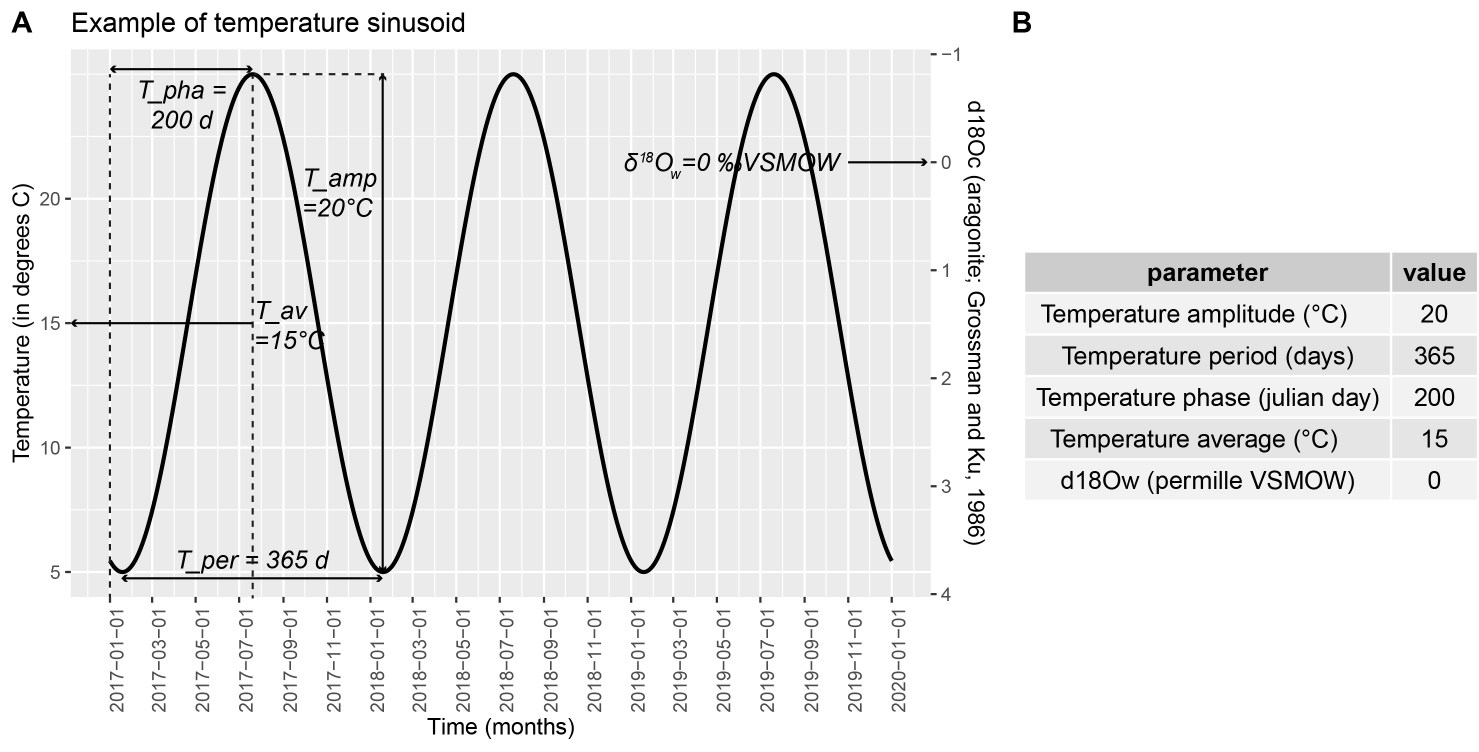
\includegraphics{man/figures/README-SSTcurve.png}
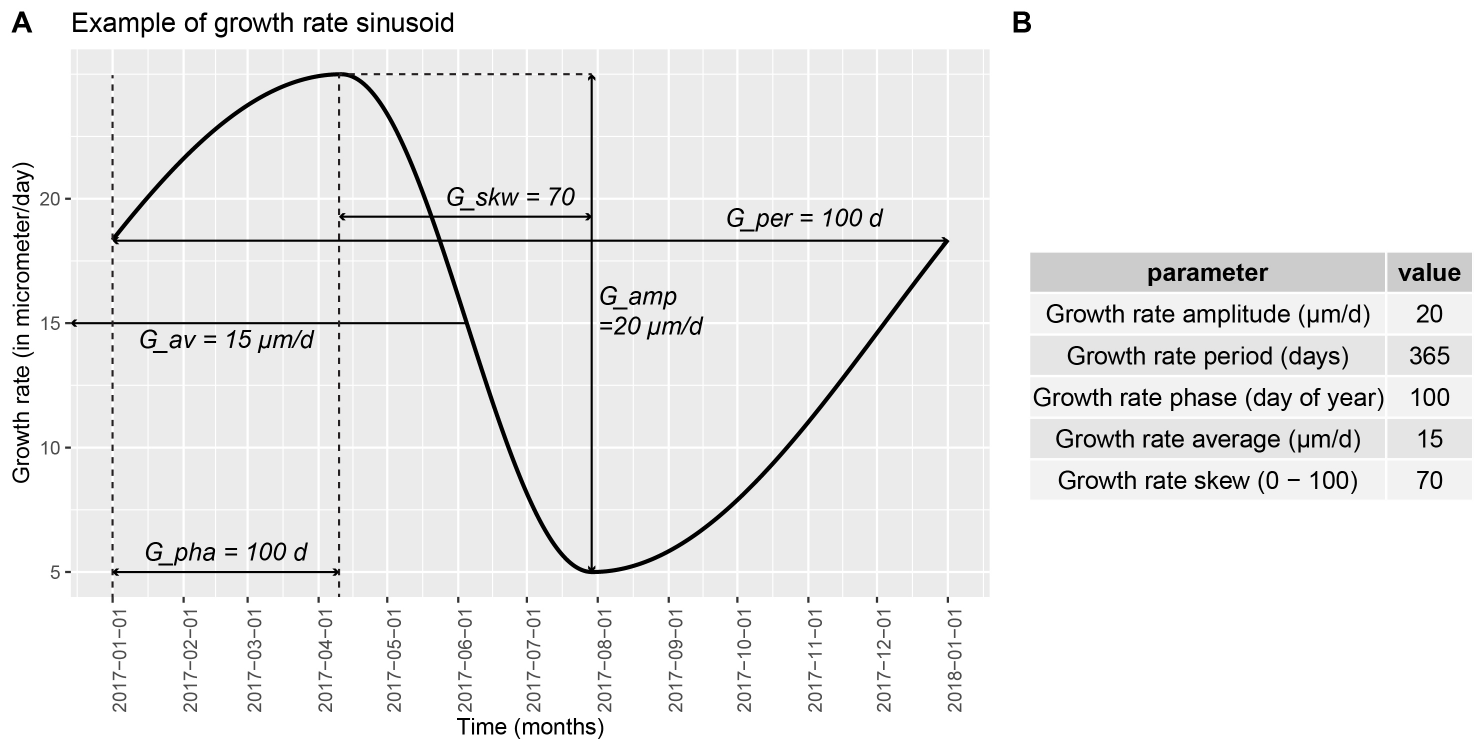
\includegraphics{man/figures/README-GRcurve.png}

The model builds on previous work by
\href{https://doi.org/10.1016/j.palaeo.2017.09.034}{Judd et al.~2018}
and expands on this previous model in several key ways:

\begin{enumerate}
\def\labelenumi{\arabic{enumi}.}
\tightlist
\item
  ShellChron allows SCEUA optimization to be carried out in a sliding
  window through the data and recognizes year transitions (see
  ``cumulative\_day()'' formula) to produce seamless age models through
  multiple years. Overlapping windows are used to estimate the
  reproducibility of model results.
\item
  ShellChron provides the option to take uncertainties on the input data
  (``D\_err'' and ``d18Oc\_err'') into account in error estimation (see
  ``mc\_err\_orth()'' and "export\_results() functions), providing
  realistic errors on the age estimation which were previously
  unsupported.
\item
  ShellChron supports different empirical formulae for converting
  temperature and d18O of the precipitation fluid into d18O records,
  providing compatibility with records consisting of various
  mineralogies (e.g.~calcite and aragonite).
\item
  ShellChron offers more dynamic input options for data on the variable
  that is not modelled (usually d18O of precipitation fluid),
  circumventing the (often false) assumption that this variable remains
  constant throughout the year and preventing fixed values for this
  variable hardcoded in the model.
\item
  ShellChron achieves more efficient SCEUA modelling by pre-guessing the
  parameters of temperature and growth rate sinusoids using a sinusoidal
  regression (see ``sinreg()'' formula). This is an essential feature
  that allows ShellChron to process more optimization windows while
  retaining competitive processing time (see Figure 3).
\end{enumerate}

\begin{figure}
\centering
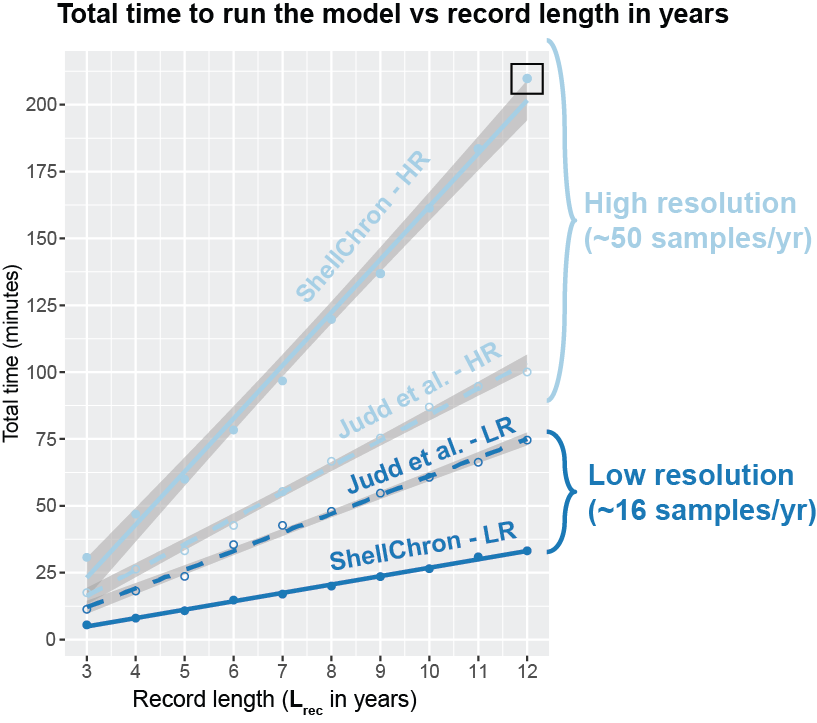
\includegraphics{man/figures/README-Timing.png}
\caption{Figure 3: Timing of whole model run at various data
resolutions}
\end{figure}

\hypertarget{installation}{%
\subsection{Installation}\label{installation}}

You can install the released version of ShellChron from
\href{https://CRAN.R-project.org}{CRAN} with:

\begin{Shaded}
\begin{Highlighting}[]
\KeywordTok{install.packages}\NormalTok{(}\StringTok{"ShellChron"}\NormalTok{)}
\end{Highlighting}
\end{Shaded}

And the development version from \href{https://github.com/}{GitHub}
with:

\begin{Shaded}
\begin{Highlighting}[]
\CommentTok{# install.packages("devtools")}
\NormalTok{devtools}\OperatorTok{::}\KeywordTok{install_github}\NormalTok{(}\StringTok{"nielsjdewinter/ShellChron"}\NormalTok{)}
\end{Highlighting}
\end{Shaded}

\hypertarget{example}{%
\subsection{Example}\label{example}}

This is a basic example which shows you how to solve a common problem:

\begin{Shaded}
\begin{Highlighting}[]
\KeywordTok{library}\NormalTok{(ShellChron)}
\CommentTok{## Full model run}
\CommentTok{# }\AlertTok{WARNING}\CommentTok{: Running the full ShellChron model (even on small example data) always takes some time (usually in the order of 30-60 minutes)}
\CommentTok{# example <- wrap_function(path = getwd(),}
\CommentTok{#  file_name = system.file("extdata", "Virtual_shell.csv",}
\CommentTok{#  package = "ShellChron"),}
\CommentTok{#  "calcite",}
\CommentTok{#  1,}
\CommentTok{#  365,}
\CommentTok{#  d18Ow = 0,}
\CommentTok{#  t_maxtemp = 182.5,}
\CommentTok{#  MC = 1000,}
\CommentTok{#  plot = FALSE,}
\CommentTok{#  plot_export = FALSE,}
\CommentTok{#  export_raw = FALSE)"}

\CommentTok{# Quick demo on how to create an SST curve}
\CommentTok{# Set parameters}
\NormalTok{T_amp <-}\StringTok{ }\DecValTok{20}
\NormalTok{T_per <-}\StringTok{ }\DecValTok{365}
\NormalTok{T_pha <-}\StringTok{ }\DecValTok{150}
\NormalTok{T_av <-}\StringTok{ }\DecValTok{15}
\NormalTok{T_par <-}\StringTok{ }\KeywordTok{c}\NormalTok{(T_amp, T_per, T_pha, T_av)}
\NormalTok{SST <-}\StringTok{ }\KeywordTok{temperature_curve}\NormalTok{(T_par, }\DecValTok{1}\NormalTok{, }\DecValTok{1}\NormalTok{) }\CommentTok{# Run the function}
\end{Highlighting}
\end{Shaded}

\end{document}
